%% analyse.tex
%% $Id: analyse.tex 61 2012-05-03 13:58:03Z bless $

\chapter{Analyse}
\label{ch:Analyse}
%% ==============================




%% ==============================
\section{Anforderungen}
%% ==============================
\label{ch:Analyse:sec:Anforderungen}

Um einen Graphen, der zur Diskussion steht auf einen Problemkern zu reduzieren können verschiedene Reduktionsregeln verwendet werden. \\
Zunächst werden die Regeln anhand der folgenden Kriterien beurteilt:
\begin{itemize}
	\item Laufzeit
	\item Erwartete Reduktion
	\item Ressourcenverbrauch
	%\item Wie gut ist das Ergebnis im Vergleich zu anderen Algorithmen?	
\end{itemize}
Dann wird die Anwendung und der Effekt der Regeln auf das eigens erstellte Testset untersucht, um folgende Fragen zu beantworten:
\begin{itemize}
\item Wie effektiv sind die Reduktionsregeln in der Anwendung?
	\begin{itemize}
		\item Wie oft sind die Regeln anwendbar?
		\item Wie viel wird reduziert?
	\end{itemize}
\item Wie (gut) funktionieren die Reduktionsregeln in Kombination?
\item Wie sehen Graphen aus, auf die keine Regel anwendbar ist?
\item Wie sehen Graphen aus, auf die genau eine Regel anwendbar ist?
\end{itemize}

%% ==============================
\section{Bewertung der Reduktionsregeln}
%% ==============================
\label{ch:Analyse:sec:Berwertung}

Um die verwendeten Reduktionsregeln zu bewerten, beziehungsweise zu vergleichen, betrachten wir auf der einen Seite die theoretisch mögliche Reduktion und auf der anderen, wie sich der implementierte Algortihmus verhält. 

%\begin{figure}[htb]
%\centering
 % 	{
\includegraphics[width=.3\textwidth]{Logo-Uni-Trier.jpg}}
%	\caption{Logo der Universität Trier.\label{fig:grafik1}}
%\centering
%\end{figure}


\begin{table}[htb]
\caption{Bewertung der Reduktionsregeln\label{tab:liste}}
\vspace*{1em}
\centering

\bgroup
\def\arraystretch{1.3}%  1 is the default, change whatever you need
\begin{threeparttable}
\begin{tabular}[c]{l|l|c}
	
	\multicolumn{1}{c|}{\textbf{Reduktionsregel}} & 
	\multicolumn{1}{c|}{\textbf{Laufzeit}} & 
	\multicolumn{1}{c}{\textbf{Reduktion}} \\ 
	
	\hline

	Nemhauser Trotter&$O(k^{3})$&  $\leq 2k$\\
	Kronenregel&$O(\sqrt{|V|}|E|)$ & $\leq 3k$\\
	Buss&$O(k|V|)$  & $\leq k^{2}$\\
	Grad 0&$O(m|V|)\ mit\ m\leq1$& \tnote{*} \\
	Grad 1&$O(m|V|)\ mit\ m<1$& \tnote{*} \\
	%Grad 2&$O(n|V|)\ mit\ n\leq1$&\\
	
\end{tabular}

\begin{tablenotes}\footnotesize
\item[*] Die Reduktion dieser Regeln hängt stark von der Struktur des Graphen ab. Eine formale Bestimmung der zu erwartenden Reduktion steht noch aus.
\item \emph{k} beschreibt jeweils den Eingabeparameter der Knotenüberdeckung für einen Graphen $G=(V,E)$
\end{tablenotes}

\end{threeparttable}

\egroup

\end{table}

In Tabelle \ref{tab:liste} stehen die Laufzeiten in der $O$-Notation und erwartete Größe der reduzierten Problemkerns der Nemhauser Trotter Regel \cite[S67]{fixed}, der Kronenregel \cite[S71]{fixed} \cite{manual}, die der Buss Regel \cite[S67]{fixed} und von einfachen Reduktionsregeln (Grad 0 und Grad 1) gegenüber. Die Laufzeiten der einfachen Reduktionsregeln ergeben sich folgt:
\begin{proof}
 Sei Graph G = (V,E)
	\begin{align*}
  		Grad\ 0-Reduktion\\
  		\underline{1.Fall:}\ |E|=0&\\
  		&jeder\ Knoten\ aus\ V\ muss\ betrachtet\ werden.\\
  		&\Rightarrow\ Laufzeit:\ O(|V|)\\  		
  		\underline{2.Fall:}\ |E|>0&\\
  		&Sobald\ bei\ der\ Iteration\ ein\ Knoten\ mit\ Grad(v)>0\ (v\in V)\ \\
  		&ausgew\ddot{a}hlt\ wird,\ k\ddot{o}nnen\ alle\ Nachbarn\ ignoriert\ werden.\\
  		&\Rightarrow\ Laufzeit:\ O(m|V|)\ mit\ (m<1)\\
	\end{align*}
\end{proof}
\begin{proof}
 Sei Graph G = (V,E)
	\begin{align*}
  		Grad\ 1-Reduktion\\
  		&Sobald\ bei\ der\ Iteration\ ein\ Knoten\ mit\ Grad(v)=1\ (v\in V)\ \\
  		&ausgew\ddot{a}hlt\ wird,\ wird\ der\ Nachbar\ in\ die\ Knotenüberdeckung\\
  		&aufgenommen.\\
  		&\Rightarrow\ Laufzeit:\ O(m|V|)\ mit\ (m<1)\\
	\end{align*}
\end{proof}

TODO was bringt die Bewertung?

%% ==============================
\section{Anwendung der Reduktionsregeln}
%% ==============================
\label{ch:Analyse:sec:Anwendung}
%% ==============================

Das Testset an dem die Algorithmen angewandt wurden besteht aus ungerichteten Graphen, die jeweils eine Knotenmenge von 1000 Knoten und eine Kantenanzahl von 1000 bis 10000 (aufsteigend in 200er Schritten) umfassen. Von jeder \emph{Graphklasse}, die sich durch die Kantenmenge auszeichnet gibt es 20 Exemplare. Dadurch entsteht ein Testset von 900 Graphen. Zum Erstellen der Graphen wurde die LEDA-Funktion \lstinline{random_simple_undirected_graph(|V|,|E|)} \cite{manual} verwendet. Da Zufallsgraphen verwendet werden, gibt es keine Vorgabe für den Parameter \emph{k}. Die obere Beschränkung der Kantenmenge (10000) hat sich bei den Tests ergeben, da ab einer bestimmten Dichte, beziehungsweise Knotenanzahl keine Reduktionsregel mehr erfolgreich ist. Dies kann mit der erwarteten Reduktion (siehe Tabelle \ref{tab:liste}) erklärt werden: Je dichter der Graph wird, desto größer wird \emph{k} und sobald $k>\frac{|V|}{2}$ ist, ist bei der Nemhauser Trotter-Regel und somit auch bei den anderen die theoretische Größe des reduzierten Problemkerns größer oder gleich der Menge der Knoten. Daher eignen sich viele Benchmarktests \footnote{http://dimacs.rutgers.edu/pub/challenge/graph/benchmarks/} \footnote{http://sites.nlsde.buaa.edu.cn/~kexu/benchmarks/graph-benchmarks.htm} nicht, was sich bei Testdurchläufen herausstellte. Die Knotenmenge 1000 erwies sich in den Tests als ausreichend hoher Wert, um das Einsetzen der Reduktionsregeln zu beobachten.\\
Die Reduktionsregeln wurden jeweils solange auf einen Graphen angewandt, bis sich keine Änderungen mehr ergeben haben. Erzielte eine der Regeln eine Reduktion, wurde der gesamte Vorgang wiederholt. Ausgeführt wurden die Experimente auf einem 2.6 GHz, Zweikern, Intel Core i5-3320M mit 8 GB Speicher. In der Tabelle \ref{tab:anwendung} werden die durchschnittliche Anzahl der Anwendungen pro Graph, die durschnittliche Reduktion (Anzahl der Knoten, die aus dem Graphen entfernt wurden), und die durchschnittliche CPU-Zeit, die pro Graph aufgebracht wurde. Die Buss Regel wurde von der Untersuchung ausgeschlossen, da kein Wert für \emph{k} vorliegt, welcher für die Anwendung essentiell ist, während die restlichen Regeln auch ohne diesen Parameter verwendbar sind.\\
Tabelle \ref{tab:anwendung} spiegelt die erwarteten Werte (\ref{tab:liste}) in soweit wieder, als das die Nemhauser Trotter Regel eine deutlich bessere Reduktion als die Kronenregel erreicht, zumindest, wenn sie isoliert angewandt wird. Dabei werden weniger Durchläufe, allerdings ein höherer Rechenaufwand benötigt. 

\begin{table}[htb]
\caption{Anwendung einzelner Reduktionsregeln\label{tab:anwendung}}
\vspace*{1em}
\centering

\bgroup
\def\arraystretch{1.3}%  1 is the default, change whatever you need


\begin{tabular}[c]{l|l|l|l}
	
	\multicolumn{1}{c|}{\textbf{Reduktionsregel}} & 
	\multicolumn{1}{c|}{\textbf{Anwendungen}} & 
	\multicolumn{1}{c|}{\textbf{Reduktion}} & 
	\multicolumn{1}{c}{\textbf{CPU-Zeit}} \\ 
	
	\hline

	Nemhauser Trotter& 0.27 &  50.3 & 0.014\\
	Kronenregel& 0.46 & 19.77 & 0.005\\
	Grad 1&1.32 & 99.06 & 0.001\\
	%Grad 2&$O(n|V|)\ mit\ n\leq1$&\\
	
\end{tabular}

\egroup

\end{table}
Während sich die Reduktion durch die Nemhauser Trotter und die Grad 1 Regel bei der Anwendung an dichteren Graphen, also Graphen mit einer höheren Kantenzahl \cite{dummy}, erwartungsgemäß stetig verringerte, zeigten sich bei der Kronenregel einige Ausnahmen. Wie in Abbildung \ref{fig:crown} zu sehen ist, setzten sich diese deutlich vom Durchschnitt ab. In Tabelle \ref{tab:crownSpecial} werden die drei Graphen mit einer Kantenmenge über (beziehungsweise gleich) 3000 und einer durch die Kronenregel erreichten Reduktion > 480 Knoten betrachtet. Keiner dieser Graphen ist bipartit.
Bei allen drei Graphen führte die Anwendung der Nemhauser Trotter Regel zu keinerlei nennenswertem Effekt, weder isoliert, noch in Kombination mit den anderen Regeln. Ähnlich verhielt sich zunächst die Grad$_{1}$ Regel, wohingegen die Anwendung in Kombination einen großen Einfluss auf die Reduktion hatte. Kombiniert man die Regeln, scheint die Reihenfolge, in der sie eingesetzt werden schwer ins Gewicht zu fallen. Besonders fiel das bei Graph$_{1}$ (3200 Kanten) auf. Wurde zuerst die Grad$_{1}$ und dann die Kronenregel verwendet, war jeweils lediglich ein Durchlauf (Anwendung) zu beobachten. Die Grad$_{1}$ Regel scheint den Graphen derart zu verändern, als dass kaum Reduktionsmöglichkeiten bei der Kronenregeln übrig bleiben. Betrachtet man dagegen das Ergebnis des Graphen$_{2}$, erzeugte die Anwendung in gerade dieser Reihenfolge eine Lösung des Problems: 1000 von 1000 Konten reduziert, wovon 619 eine Knotenüberdeckung für den Graphen$_{2}$ bilden. Auch hier war die Reihenfolge wieder wichtig, wie man bei der Reduktionsmenge beim entgegengesetzten Experiment (erst Kronenregel, dann Grad$_{1}$ Regel) sieht, wo 858 Knoten entfernt wurden. Bei Graph$_{1}$ und Graph$_{3}$ zeichnet sich der übrig gebliebene Problemkern nach der jeweils größten Reduktion dadurch aus, dass der Großteil der Knoten vom Grad 2 ist. Der Problemkern $G'_{3}$ von Graph$_{3}$ lässt sich in die Knotenmengen $V_{1}$ und $V_{2}$  mit $|V_{1}| = |V_{2}| = 5$ aufteilen. Bis auf die Knoten $v_{1} \in V_{1}$ und $v_{2} \in V_{2}$, welche vom Grad 3 sind, hat jeder andere Knoten in  $G'_{3}$ (durch die vorherige Reduktion) den Grad 2. Für  $v_{1}$ und $v_{2}$ existiert eine Kante $(v_{1}, v_{2})$ in $G'_{3}$, welche die Knotenmengen verbindet. Innerhalb der Knotenmengen existiert einen Zyklus (Kreis) \cite{dummy}, mit ungerader Knotenzahl, woraus sich folgern lässt, dass $G'_{3}$ nicht bipartit ist. Hier ist keine der Reduktionsregeln mehr erfolgreich.

\begin{figure}[htb]
\centering
  	{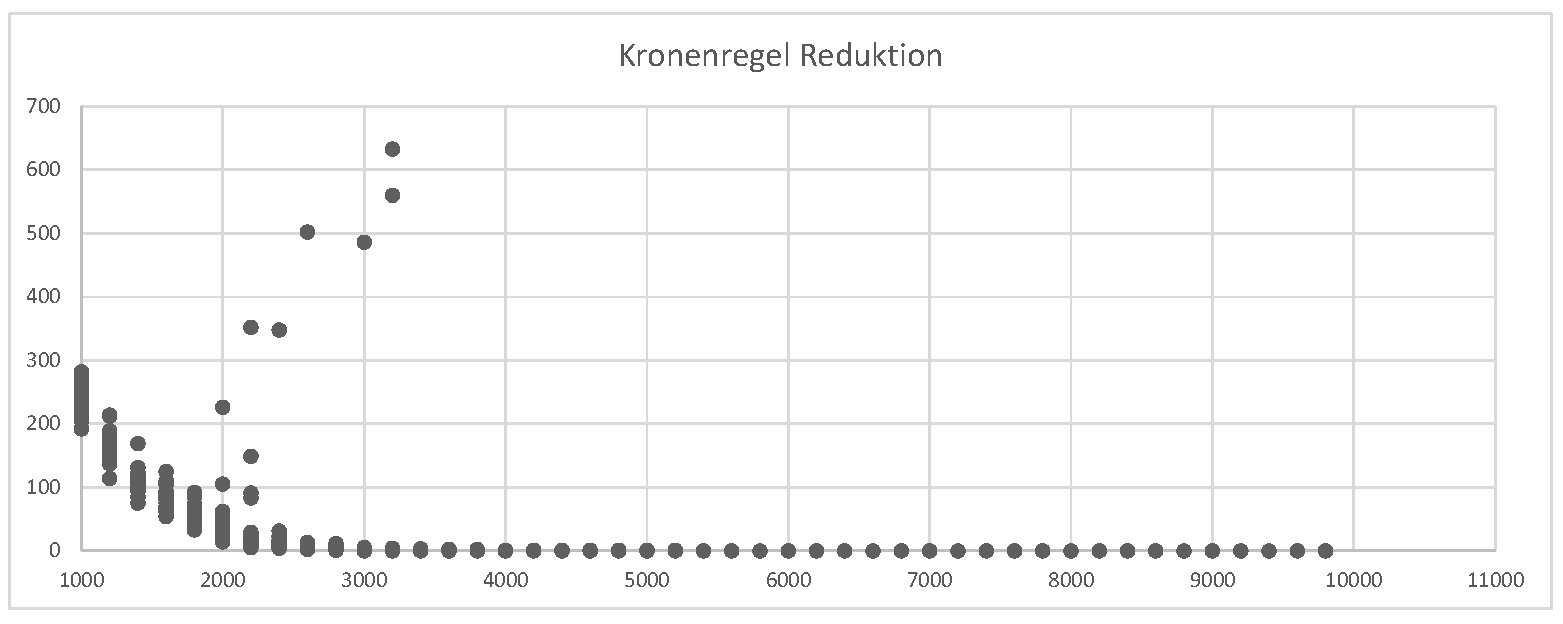
\includegraphics[width=\textwidth]{analysisCrown.pdf}}
	\caption{Anwendung der Kronenregel.\label{fig:crown}}
\centering
\end{figure}

\begin{table}[htb]
\caption{Besondere Graphen für die Kronenregel \label{tab:crownSpecial}}
\vspace*{1em}
\centering

\bgroup
\def\arraystretch{1.3}%  1 is the default, change whatever you need

\begin{threeparttable}

\begin{tabular}[c]{l|l|l|l|l}
	
	\multicolumn{1}{c|}{\textbf{Graph}} & 
	\multicolumn{1}{c|}{\textbf{Reduktionsregeln}} & 
	\multicolumn{1}{c|}{\textbf{Anwendungen$_{1}$}} &
	\multicolumn{1}{c|}{\textbf{Anwendungen$_{2}$}} &
	\multicolumn{1}{c}{\textbf{Reduktion}} \\ 
	
	\hline
		
	Graph$_{1}$ & Kronenregel& 11 & - & 560\\
	& Nemhauser Trotter & 1 & - & 4\\
	& Grad$_{1}$ & 1 & - & 18 \\
	& Grad$_{1}$-Kronenregel & 1 & 1 & 22\\
	& Kronenregel - Grad$_{1}$ & 14 & 11 & 946\\
	
	\hline

	Graph$_{2}$ & Kronenregel & 13 & - & 486\\
	& Nemhauser Trotter & 1 & - & 6\\
	& Grad$_{1}$ & 2 & - & 40 \\
	& Grad$_{1}$-Kronenregel & 12 & 13 & 1000\\
	& Kronenregel - Grad$_{1}$ & 18 & 12 & 858\\

	\hline	
	
	Graph$_{3}$ & Kronenregel & 15 & - &633\\	
	& Nemhauser Trotter & 1 & - & 4\\
	& Grad$_{1}$ & 2 & - & 46 \\
	& Grad$_{1}$-Kronenregel & 18 & 11 & 990\\
	& Kronenregel - Grad$_{1}$ & 15 & 9 & 971\\
	


	
	
\end{tabular}
\begin{tablenotes}\footnotesize
\item EINFÜGEN
\end{tablenotes}

\end{threeparttable}

\egroup

\end{table}

Werden die Reduktionsregeln in Kombination angewandt, zeigen sich sowohl durch verschiedene Kombinationen, als auch durch unterschiedliche Reihenfolge  im Ergebnis große Unterschiede.

\begin{table}[htbp]
\caption{Anwendung kombinierter Reduktionsregeln\label{tab:kombination}}
\vspace*{1em}
\centering

\bgroup
\def\arraystretch{1.3}%  1 is the default, change whatever you need


\begin{tabular}[c]{l|l|l|l|l}
	
	\multicolumn{1}{c|}{\textbf{Kombination}} &
	\multicolumn{1}{c|}{\textbf{Anwendungen$_{1}$}} &
	\multicolumn{1}{c|}{\textbf{Anwendungen$_{2}$}} &
	\multicolumn{1}{c|}{\textbf{Anwendungen$_{3}$}} & 
	\multicolumn{1}{c}{\textbf{Reduktion}} \\
	\hline

	K - G$_{1}$ & 3.63 & 4.3 & - &331.8\\
	G$_{1}$ - K & 4.37 & 3.22 & - &331.17\\
	K - NT & 0.8 & 0.38 & - & 68.28 \\
	NT - K & 0.45 & 0.56 & - & 68.6\\
	G$_{1}$ - NT & 1.33 & 0.017 & - & 99.87\\
	NT - G$_{1}$ & 0.28 & 1.13 & - & 99.87\\
	K  - G$_{1}$ - NT & 3.61 & 4.29 & 0.11 & 334.67 \\
	K - NT - G$_{1}$ & 3.6 & 0.87 & 3.39 & 334.83 \\
	G$_{1}$ - NT - K & 4.36 & 0.12 & 3.2 & 334.17 \\
	G$_{1}$ - K - NT & 3.61 & 3.2 & 0.65 & 334.16 \\
	NT - K - G$_{1}$ & 0.39 & 3.44 & 4.03 & 335.2 \\
	NT - G$_{1}$ - K & 0.91 & 3.42 & 3.2 & 334.16 \\

	
\end{tabular}

\egroup

\end{table}


%% ==============================
\section{Interpretation der Ergebnisse}
%% ==============================
\label{ch:Analyse:sec:Interpretation}
%% ==============================




\section{Zusammenfassung}
%% ==============================
\label{ch:Analyse:sec:zusammenfassung}

Am Ende sollten ggf. die wichtigsten Ergebnisse nochmal in \emph{einem}
kurzen Absatz zusammengefasst werden.

%%% Local Variables: 
%%% mode: latex
%%% TeX-master: "thesis"
%%% End: 
